%\documentclass[11pt]{beamer}
\documentclass[11pt, handout]{beamer}

% Allgemeine Definitionen
\usepackage[english]{babel}	% Deutsche Sprachanpassung, z.B. Silbentrennung bei Worten mit Sonderzeichen
\usepackage[utf8]{inputenc}		% Direkte Eingabe von Umlauten

\usepackage{multimedia}		% Animations-Unterstützung (braucht hyperref | hyperref ist Teil von beamer )
\usepackage{xcolor}
\usepackage{fancyvrb}


% Verschiedene Operatoren
\newcommand{\union}{\ensuremath{\cup}}		% Die Vereinigung
\newcommand{\schnitt}{\ensuremath{\cap}}		% Der Schnitt
\newcommand{\und}{\ensuremath{\wedge}}		% Das und-Symbol
\newcommand{\oder}{\ensuremath{\vee}}		% Das oder-Symbol
\newcommand{\folgt}[1]{\ensuremath{\stackrel{#1}{\Rightarrow}}}	% Das Folgerungszeichen mit Symbol darüber 
\newcommand{\gleich}[1]{\ensuremath{\stackrel{#1}{=}}}	% Das Gleichheitszeichen mit Symbol darüber 
\newcommand{\isdef}{\ensuremath{\mathrel{\mathop:}=}}		% Das "ist-definiert"-Zeichen
\newcommand{\defis}{\ensuremath{=\mathrel{\mathop:}}}		% Das "ist-definiert"-Zeichen (andersrum)

% Weiterer nützlicher Kram
%\usepackage{enumitem}		% NICHT kompatibel mit beamer!
\usepackage{amsfonts, amsmath, amssymb}
\usepackage{amsthm}			% Eigene Umgebungen
\usepackage{thumbpdf}	% Seitenvorschau in PDF-Dokumenten

\usepackage{nicefrac}

\usepackage{pgf, tikz}
\usetikzlibrary{arrows, decorations.pathreplacing, calc, decorations.pathmorphing, shapes}

% Erst die Farbe (optional), dann die Norm, dann der Inhalt
\newcommand{\norm}[3][black]{\ensuremath{\left\Vert #3\right\Vert_{\textcolor{#1}{#2}}}}

% Die folgenden Befehle dienen dazu, verschiedene Konventionen darzustellen. Man kann damit
% auf einfache Weise die in dem Dokument verwendeten Konventionen umschalten.

%\newcommand{\bisn}[1]{\ensuremath{\underline{#1}}}	% Bezeichnung für die Menge {1,..,n}
\newcommand{\bisn}[1]{\ensuremath{\{1,\dots , #1 \}}}	% Alternative (ohne Fallunterscheidung)

% Das Erzeugnis, das erste Argument zeigt an, welches Erzeugnis gemeint ist, das zweite gibt seinen Inhalt an.
%\newcommand{\spn}[2][]{\ensuremath{\mathrm{span} \{ #1 \}}}
\newcommand{\spn}[2][]{\ensuremath{\left\langle #2 \right\rangle _{ #1 }}}

\newcommand{\grad}[1]{\ensuremath{\mathrm{grad}( #1 )}}
%\newcommand{\grad}[1]{\ensuremath{\nabla #1}}

\newcommand{\tr}[1]{\ensuremath{#1^{tr}}} % Bezeichnung für die Transponierte einer Matrix

% Die Mengentheoretische Differenz
\newcommand{\ohne}{\ensuremath{-}}
%\newcommand{\ohne}{\ensuremath{\backslash}}

\DeclareMathOperator{\Hom}{Hom}
\DeclareMathOperator{\GL}{GL}
\DeclareMathOperator{\diag}{diag}
\DeclareMathOperator{\Rg}{Rang}
\DeclareMathOperator{\Bild}{Bild}
\DeclareMathOperator{\Kern}{Kern}
\DeclareMathOperator{\Spur}{Spur}
\DeclareMathOperator{\Aut}{Aut}
\DeclareMathOperator{\Sym}{Sym}
\DeclareMathOperator{\Pot}{Pot}
\DeclareMathOperator{\Grad}{Grad}
\DeclareMathOperator{\kgV}{kgV}

\newcommand{\menge}[1]{\ensuremath{\mathbb{#1}}}
\newcommand{\N}{\menge{N}}
\newcommand{\Z}{\menge{Z}}
\newcommand{\Q}{\menge{Q}}
\newcommand{\R}{\menge{R}}
\newcommand{\C}{\menge{C}}

% Mit den schönen Buchstaben arbeiten
\renewcommand{\phi}{\varphi}

\renewcommand{\subset}{\subseteq}

% Verschiedene mögliche Umgebungen
\newtheorem{lem}{Lemma}[section]		% Lemma
\newtheorem{bsp}[lem]{Beispiel}		% Beispiel
\newtheorem{folg}[lem]{Folgerung}	% Folgerung
\newtheorem{bem}[lem]{Bemerkung}
\newtheorem{satz}[lem]{Satz}			% Satz
\newtheorem{kor}[lem]{Korollar}		% Korollar
%\newtheorem{alg}[lem]{Algorithmus}	% Algorithmus
%\theoremstyle{definition}
\newtheorem{defi}[lem]{Definition}	% Definition
\theoremstyle{remark}
\newtheorem*{idea}{Beweisidee}	% Beweisidee (vor dem eigentlichen Beweis)




\beamertemplatenavigationsymbolsempty

\usetheme{Madrid}
%	AnnArbor | Antibes | Bergen |
%	Berkeley | Berlin | Boadilla |
%	boxes | CambridgeUS | Copenhagen |
%	Darmstadt | default | Dresden |
%	Frankfurt | Goettingen |Hannover |
%	Ilmenau | JuanLesPins | Luebeck |
%	Madrid | Malmoe | Marburg |
%	Montpellier | PaloAlto | Pittsburgh |
%	Rochester | Singapore | Szeged |
%	Warsaw
%\usecolortheme{seahorse}
%	albatross | beaver | beetle |
%	crane | default | dolphin |
%	dove | fly | lily | orchid |
%	rose |seagull | seahorse |
%	sidebartab | structure |
%	whale | wolverine
%\usefonttheme{professionalfonts}
%	default | professionalfonts | serif |
%	structurebold | structureitalicserif |
%	structuresmallcapsserif
%\useinnertheme{rounded}
%	circles | default | inmargin |
%	rectangles | rounded
%\useoutertheme{shadow}
%	default | infolines | miniframes |
%	shadow | sidebar | smoothbars |
%	smoothtree | split | tree

% Graphic support
\newcommand{\primaryBlue}{blue}
\newcommand{\primaryRed}{red}
\newcommand{\primaryGreen}{green!60!black}


\newcommand{\colorVertex}{\primaryBlue}
\newcommand{\colorEdge}{black}
\newcommand{\colorFace}{yellow}
\newcommand{\colorEdgeBack}{\primaryBlue!20!white}

\newcommand{\colorVertexNode}{magenta!50!white}

\newcommand{\colorEdgeA}{\primaryBlue}
\newcommand{\colorEdgeB}{\primaryRed}
\newcommand{\colorEdgeC}{\primaryGreen}


\newcommand{\colorFaceA}{cyan}
\newcommand{\colorFaceB}{magenta}
\newcommand{\colorFaceC}{orange}

\newcommand{\colorRed}{\primaryRed}

\newcommand{\colorGraphA}{black}
\newcommand{\colorGraphB}{\primaryBlue}
\newcommand{\colorGraphC}{\primaryRed}

\newcommand{\colorGraphAlpha}{\primaryRed}
\newcommand{\colorGraphBeta}{black}
\newcommand{\colorGraphGamma}{\primaryBlue}
\newcommand{\colorGraphDelta}{\primaryGreen}

% This document contains the TikZ-header for all our LaTeX-computations.
% It especially contains all global graphic parameters.

\usepackage{amsmath, amssymb, amsfonts} % Standard Math-stuff

\usepackage{tikz}
\usetikzlibrary{calc}
\usetikzlibrary{positioning}

% Define a text=none option for nodes that ignores the given text, from
% https://tex.stackexchange.com/questions/59354/no-text-none-in-tikz
\makeatletter
\newif\iftikz@node@phantom
\tikzset{
  phantom/.is if=tikz@node@phantom,
  text/.code=%
    \edef\tikz@temp{#1}%
    \ifx\tikz@temp\tikz@nonetext
      \tikz@node@phantomtrue
    \else
      \tikz@node@phantomfalse
      \let\tikz@textcolor\tikz@temp
    \fi
}
\usepackage{etoolbox}
\patchcmd\tikz@fig@continue{\tikz@node@transformations}{%
  \iftikz@node@phantom
    \setbox\pgfnodeparttextbox\hbox{}
  \fi\tikz@node@transformations}{}{}
\makeatother

% Now we define the global styles
% The global styles are defined nestedly. You have to give your tikzpicture
% the global options [vertexStyle, edgeStyle, faceStyle] to activate them.
% 
% You can disable labels by using the option nolabels, i.e. 
% vertexStyle=nolabels to deactivate vertex labels.
%
% If you want to have a specific style for your picture, you can also use
% this specific meta-style instead of the general style. For example if you
% want to use double edges in one single picture - no matter the style of
% the rest of the document - you can use edgeDouble instead of edgeStyle.
%
% To set the default style, modify the vertexStyle/.default entry.

% Vertex styles
\tikzset{ 
    vertexNodePlain/.style = {fill=gray, shape=circle, inner sep=0pt, minimum size=2pt, text=none},
    vertexPlain/labels/.style = {
        vertexNode/.style={vertexNodePlain},
        vertexLabel/.style={gray}
    },
    vertexPlain/nolabels/.style = {
        vertexNode/.style={vertexNodePlain},
        vertexLabel/.style={text=none}
    },
    vertexPlain/.style = vertexPlain/#1,
    vertexPlain/.default=labels
}
\tikzset{
    vertexNodeNormal/.style = {fill=blue, shape=circle, inner sep=0pt, minimum size=4pt, text=none},
    vertexNormal/labels/.style = {
        vertexNode/.style={vertexNodeNormal},
        vertexLabel/.style={blue}
    },
    vertexNormal/nolabels/.style = {
        vertexNode/.style={vertexNodeNormal},
        vertexLabel/.style={text=none}
    },
    vertexNormal/.style = vertexNormal/#1,
    vertexNormal/.default=labels
}
\tikzset{
    vertexNodeBall/.style = {shape=circle, ball color=orange, inner sep=2pt, outer sep=0pt, minimum size=3pt},
    vertexBall/labels/.style = {
        vertexNode/.style={vertexNodeBall, text=black},
        vertexLabel/.style={text=none}
    },
    vertexBall/nolabels/.style = {
        vertexNode/.style={vertexNodeBall, text=none},
        vertexLabel/.style={text=none}
    },
    vertexBall/.style = vertexBall/#1,
    vertexBall/.default=labels
}
\tikzset{ 
    vertexStyle/.style={vertexNormal=#1},
    vertexStyle/.default = labels
}


% 1) position of the vertex
% 2) relative position of the node
% 3) name of the vertex
\newcommand{\vertexLabelR}[3]{
    \node[vertexLabel, #2] at (#1) {#3};
}
% 1) position of the vertex
% 2) absolute position of the node
% 3) name of the vertex
\newcommand{\vertexLabelA}[3]{
    \node[vertexLabel] at (#2) {#3};
}


% Edge styles
% If you have trouble with the double-lines overlapping, this might (?) help:
% https://tex.stackexchange.com/questions/288159/closing-the-ends-of-double-line-in-tikz
\tikzset{
    edgeLinePlain/.style={line join=round},
    edgePlain/labels/.style = {
        edge/.style={edgeLinePlain},
        edgeLabel/.style={fill=blue!20!white}
    },
    edgePlain/nolabels/.style = {
        edge/.style={edgeLinePlain},
        edgeLabel/.style={text=none}
    },
    edgePlain/.style = edgePlain/#1,
    edgePlain/.default = labels
}
\tikzset{
    edgeLineDouble/.style = {thin, double=gray!90!white, double distance=.3pt, line join=round},
    edgeDouble/labels/.style = {
        edge/.style = {edgeLineDouble},
        edgeLabel/.style = {fill=blue!20!white}
    },
    edgeDouble/nolabels/.style = {
        edge/.style = {edgeLineDouble},
        edgeLabel/.style = {text=none}
    },
    edgeDouble/.style = edgeDouble/#1,
    edgeDouble/.default = labels
}
\tikzset{
    edgeStyle/.style = {edgePlain=#1},
    edgeStyle/.default = labels
}

% Face styles
% Here we have an exception - the style face is always defined.
% 
\newcommand{\faceColorY}{yellow!60!white}   % yellow
\newcommand{\faceColorB}{blue!60!white}     % blue
\newcommand{\faceColorP}{cyan!60}           % purple
\newcommand{\faceColorR}{red!60!white}      % red
\newcommand{\faceColorG}{green!60!white}    % green
\newcommand{\faceColorO}{orange!50!yellow!70!white} % orange

\newcommand{\faceColor}{\faceColorY}
\newcommand{\faceColorSwap}{\faceColorB}
\tikzset{
    face/.style = {fill=#1},
    face/.default = \faceColor,
    faceY/.style = {face=\faceColorY},
    faceB/.style = {face=\faceColorB},
    faceP/.style = {face=\faceColorP},
    faceR/.style = {face=\faceColorR},
    faceG/.style = {face=\faceColorG},
    faceO/.style = {face=\faceColorO}
}
\tikzset{
    faceStyle/labels/.style = {
        faceNode/.style = {}
    },
    faceStyle/nolabels/.style = {
        faceNode/.style = {text=none}
    },
    faceStyle/.style = faceStyle/#1,
    faceStyle/.default = labels
}
\tikzset{ face/.style={fill=#1} }
\tikzset{ faceSwap/.code=
    \ifdefined\swapColours
        {face=\faceColorSwap}
    \else
        {face=\faceColor}
    \fi
}

% Sometimes we want to implement different behaviour for the generated 
% HTML-pictures (for example, shading is not supported in HTML).
% For that we define a macro to check whether we run the code with
% htlatex. The code comes from 
% https://tex.stackexchange.com/questions/93852/what-is-the-correct-way-to-check-for-latex-pdflatex-and-html-in-the-same-latex
\makeatletter
\edef\texforht{TT\noexpand\fi
  \@ifpackageloaded{tex4ht}
    {\noexpand\iftrue}
    {\noexpand\iffalse}}
\makeatother


\usepackage{hyperref}



\author[Baumeister]{Markus Baumeister\\ \vspace{1mm} \small{(j/w Alice Niemeyer)}}
\title{Simplicial surfaces in GAP}
\institute[Aachen]{Lehrstuhl B für Mathematik\\RWTH Aachen University}
\date{30.08.2017}

\begin{document}

% Titelseite
\begin{frame}
\titlepage
\end{frame}

\begin{frame}{Basic data}
    \begin{itemize}
        \pause
        \item Package name: \texttt{SimplicialSurfaces}
            \begin{itemize}
                \pause
                \item Not yet generally available
            \end{itemize}
        \pause
        \item Authors: Alice Niemeyer, Markus Baumeister
        \pause
        \item based on current work at Lehrstuhl B, notably Wilhelm Plesken
        \pause
        \item Internally used packages (not documentation):
            \begin{itemize}
                \pause
                \item \texttt{AttributeScheduler} by Sebastian Gutsche
                \pause
                \item \texttt{Digraphs} by De Beule, Mitchell, Pfeiffer, Wilson et al.
            \end{itemize}
    \end{itemize}
\end{frame}


\begin{frame}
    \tableofcontents[pausesections]
\end{frame}


%%%%%%%%%%%%%%%%%%%%%%%%%%%%%%%%%%%%%%%%%%%%%%%%%%%
%%
%%    First section
%%
\section{General simplicial surfaces}
\frame{\tableofcontents[currentsection]}

\begin{frame}{\uncover<3->{Triangular complexes}}
    We want to describe different structures:
    \uncover<2->{
        \begin{center}
            \begin{tikzpicture}[scale=2]
    \begin{scope}[scale=0.5,yshift=0.8cm]
                    % Coordinates of octahedron
                \def\len{2} % The length of the base
                \def\h{0.9}   % \h*\len is the hight of the apex above the 
                            % center of the square
                \coordinate (Mid) at (0,0);
                \coordinate (Right) at (0.5*\len,0.3*\len);
                \coordinate (Left) at (-0.75*\len,0.25*\len);
                \coordinate (Back) at ($(Right)+(Left)$);
                \coordinate (Center) at ($(Left)!0.5!(Right)$);
                \coordinate (Up) at ($(Center)+(0,\h*\len)$);
                \coordinate (Down) at ($(Center)+(0,-\h*\len)$);

                \filldraw[face] (Up) -- (Mid) -- (Left) -- cycle;
                \filldraw[face] (Up) -- (Mid) -- (Right) -- cycle;
                \filldraw[face] (Down) -- (Mid) -- (Left) -- cycle;
                \filldraw[face] (Down) -- (Mid) -- (Right) -- cycle;
                \draw[dashed] (Up) -- (Back) -- (Down);
                \draw[dashed] (Left) -- (Back) -- (Right);

 

    \end{scope}
    
    \begin{scope}[xshift=1cm]
        			    \coordinate (A) at (0,0);
			    \coordinate (B) at (1.7,0.5);
			    \coordinate (C) at (1.3,1.4);
			    \coordinate (D) at (0.5,1.5);
			    \coordinate (E) at (1,0.7);
			
			    % Take care to draw the faces in the back first
                            \draw[face,edge]
                                (A) -- (B) -- (C) -- cycle
                                (A) -- (C) -- (D) -- cycle;
                            \draw[face,edge]
                                (A) -- (B) -- (E) -- cycle
                                (A) -- (E) -- (D) -- cycle;
                            \draw[edge, dashed] (A) -- (C);

    \end{scope}

    \begin{scope}[xshift=3.5cm]
        			    \coordinate (A) at (0,0);
			    \coordinate (B) at (1.3,0.4);
			    \coordinate (C) at (0.4,1.3);
			
			    \filldraw[face] (A) -- (B) to[bend right=45] (C) -- cycle;
			    \filldraw[face] (A) -- (B) to[bend left=45] (C) -- cycle;


    \end{scope}
\end{tikzpicture}


        \end{center}
    }
    \uncover<3->{
        $\leadsto$ \textbf{triangular complexes}
    }
    \begin{itemize}
        \item<4-> sets of vertices, edges and faces
        \item<5-> incidence relation between them
        \item<6-> every face is a triangle
        \item<7-> every vertex lies in an edge \uncover<8->{and every edge lies in a face}
    \end{itemize}
\end{frame}


\begin{frame}{Isomorphism testing}
    Incidence structure can be interpreted as a coloured graph:
    \begin{center}
        \begin{tikzpicture}[vertexNode/.style={circle,fill=\colorVertexNode},node distance=0.5,
                faceNode/.style={fill=\faceColor,regular polygon, regular polygon sides=3}]
            \def\len{1.5}
            
            \uncover<4->{
                \coordinate[label={[vertex]left:5}] (A) at (0,0);
                \coordinate[label={[vertex]above:6}] (B) at (\len,\len);
                \coordinate[label={[vertex]below:7}] (C) at (\len,-\len);
            }
            \uncover<7->{
                \coordinate[label={[vertex]right:11}] (D) at (2*\len,0);
            }

            \uncover<2->{
                \filldraw[face] (A) -- (B) -- (C) -- cycle;
                \node at (barycentric cs:A=1,B=1,C=1) {1};
            }
            \uncover<5->{
                \filldraw[face] (B) -- (C) -- (D) -- cycle;
                \node at (barycentric cs:B=1,C=1,D=1) {8};
            }

            \uncover<3->{
                \drawEdge{A}{B}{2}
                \drawEdge{A}{C}{3}
                \drawEdge{B}{C}{4}
            }
            \uncover<6->{
                \drawEdge{B}{D}{9}
                \drawEdge{C}{D}{10}
            }

            \uncover<4->{
                \fill[vertex] (A) circle (\vSize);
                \fill[vertex] (B) circle (\vSize);
                \fill[vertex] (C) circle (\vSize);
            }
            \uncover<7->{
                \fill[vertex] (D) circle (\vSize);
            }


            \begin{scope}[xshift=5cm]
                \uncover<3->{
                    \node[edgeBackground] (E1) {2};
                    \node[edgeBackground] (E2) [right=of E1] {3};
                    \node[edgeBackground] (E3) [right=of E2] {4};
                }
                \uncover<6->{
                    \node[edgeBackground] (E4) [right=of E3] {9};
                    \node[edgeBackground] (E5) [right=of E4] {10};
                }

                \uncover<2->{
                    \node[faceNode] (F1) [above=of E2] {1}; 
                }
                \uncover<5->{
                    \node[faceNode] (F2) [above=of E4] {8};
                }

                \uncover<4->{
                    \node[vertexNode] (V1) [below=of E1] {5}
                        edge (E1) edge (E2);
                    \node[vertexNode] (V2) [right=of V1] {6}
                        edge (E1) edge (E3);
                    \node[vertexNode] (V3) [right=of V2] {7}
                        edge (E2) edge (E3);
                }
                \uncover<7->{
                    \node[vertexNode] (V4) [right=of V3] {11}
                        edge (E4) edge (E5);
                }

                \uncover<3->{
                    \draw (F1) -- (E1);
                    \draw (F1) -- (E2);
                    \draw (F1) -- (E3);
                }

                \uncover<5->{
                    \draw (F2) -- (E3);
                }

                \uncover<6->{
                    \draw (F2) -- (E4) -- (V2);
                    \draw (F2) -- (E5) -- (V3);
                }
            \end{scope}
        \end{tikzpicture}
    \end{center}

    \uncover<8->{
        $\leadsto$ reduce to graph isomorphism problem
    }

    \uncover<9->{
        $\leadsto$ can be solved quite easily by \texttt{Nauty} (McKay, Piperno)
    }

    \uncover<10->{
        Interfaced by NautyTracesInterface (by Gutsche, Niemeyer, Schweitzer)
        \begin{itemize}
            \item<11-> direct C--interface without writing files
            \item<12-> also returns automorphism group
        \end{itemize}
    }
\end{frame}


\begin{frame}{General properties}
    \pause
    Some properties can be computed for all triangular complexes:
    \pause
    \begin{itemize}
        \item Connectivity
        \pause
        \item Euler--Characteristic
    \end{itemize}
    \pause
    \textit{Orientability} is \textbf{not} one of them.
    \pause
    Counterexample:
        \begin{center}
            \begin{tikzpicture}
                \coordinate (A) at (0,0);
\coordinate (B) at (0,1.5);
\coordinate (C) at (-0.7,0.4);
\coordinate (D) at (0.8,0.4);
\coordinate (E) at (0.9,0.8);
			
\draw[edge, face]
    (A) -- (B) -- (E) -- cycle;
\draw[edge,face]
    (A) -- (B) -- (C) -- cycle
    (A) -- (B) -- (D) -- cycle;
\draw[edge, dashed] (A) -- (E);
		     

	    \end{tikzpicture}
        \end{center}
    \pause
    $\Rightarrow$ every edge lies in at most two faces (for well--definedness)
    
    \pause
    $\leadsto$ \textbf{ramified simplicial surfaces}
\end{frame}


\begin{frame}{Why ramified?}
    \pause
    Typical example of ramified simplicial surface:
    \pause
    \begin{center}
        \begin{tikzpicture}
            \begin{tikzpicture}[vertexBall, edgeDouble, faceStyle, scale=2]

% Define the coordinates of the vertices
\coordinate (V1_1) at (0., 0.);
\coordinate (V2_1) at (1., 0.);
\coordinate (V3_1) at (-0.5, 0.8660254037844384);
\coordinate (V3_2) at (1.5, 0.8660254037844388);
\coordinate (V4_1) at (0.4999999999999999, 0.8660254037844386);
\coordinate (V5_1) at (0.5000000000000001, -0.8660254037844386);
\coordinate (V5_2) at (-0.9999999999999996, 0.);
\coordinate (V5_3) at (2., 0.);


% Fill in the faces
\fill[face]  (V2_1) -- (V4_1) -- (V1_1) -- cycle;
\node[faceLabel] at (barycentric cs:V2_1=1,V4_1=1,V1_1=1) {$1$};
\fill[face]  (V2_1) -- (V3_2) -- (V4_1) -- cycle;
\node[faceLabel] at (barycentric cs:V2_1=1,V3_2=1,V4_1=1) {$2$};
\fill[face]  (V4_1) -- (V3_1) -- (V1_1) -- cycle;
\node[faceLabel] at (barycentric cs:V4_1=1,V3_1=1,V1_1=1) {$3$};
\fill[face]  (V1_1) -- (V5_1) -- (V2_1) -- cycle;
\node[faceLabel] at (barycentric cs:V1_1=1,V5_1=1,V2_1=1) {$4$};
\fill[face]  (V3_1) -- (V5_2) -- (V1_1) -- cycle;
\node[faceLabel] at (barycentric cs:V3_1=1,V5_2=1,V1_1=1) {$5$};
\fill[face]  (V2_1) -- (V5_3) -- (V3_2) -- cycle;
\node[faceLabel] at (barycentric cs:V2_1=1,V5_3=1,V3_2=1) {$6$};


% Draw the edges
\draw[edge] (V2_1) -- node[edgeLabel] {$1$} (V1_1);
\draw[edge] (V1_1) -- node[edgeLabel] {$2$} (V3_1);
\draw[edge] (V1_1) -- node[edgeLabel] {$3$} (V4_1);
\draw[edge] (V5_1) -- node[edgeLabel] {$4$} (V1_1);
\draw[edge] (V1_1) -- node[edgeLabel] {$4$} (V5_2);
\draw[edge] (V3_2) -- node[edgeLabel] {$5$} (V2_1);
\draw[edge] (V4_1) -- node[edgeLabel] {$6$} (V2_1);
\draw[edge] (V2_1) -- node[edgeLabel] {$7$} (V5_1);
\draw[edge] (V5_3) -- node[edgeLabel] {$7$} (V2_1);
\draw[edge] (V3_1) -- node[edgeLabel] {$8$} (V4_1);
\draw[edge] (V4_1) -- node[edgeLabel] {$8$} (V3_2);
\draw[edge] (V5_2) -- node[edgeLabel] {$9$} (V3_1);
\draw[edge] (V3_2) -- node[edgeLabel] {$9$} (V5_3);


% Draw the vertices
\vertexLabelR{V1_1}{left}{$1$}
\vertexLabelR{V2_1}{left}{$2$}
\vertexLabelR{V3_1}{left}{$3$}
\vertexLabelR{V3_2}{left}{$3$}
\vertexLabelR{V4_1}{left}{$4$}
\vertexLabelR{V5_1}{left}{$5$}
\vertexLabelR{V5_2}{left}{$5$}
\vertexLabelR{V5_3}{left}{$5$}

\end{tikzpicture}

        \end{tikzpicture}
    \end{center}
    \pause
    $\Rightarrow$ It is not a surface -- there is a \textit{ramification} at 
        the central vertex
    
    \pause
    A \textbf{simplicial surface} does not have these ramifications.
\end{frame}


\begin{frame}{Classification}
    \pause
    Plesken/Strzelczyk classified all closed simplicial surfaces up to 20 triangles.

    \begin{itemize}
        \pause
        \item only interesting for those without a 3--cycle of edges
        \pause
        \item e.\,g. there are 87 non--isomorphic surfaces with 20 triangles
        \pause
        \item e.\,g. there is only one surface with 10 triangles:
    \end{itemize}

    \pause
    \begin{center}
        \begin{tikzpicture}
            TODO
        \end{tikzpicture}
    \end{center}
\end{frame}


\begin{frame}{Progress report of simplicial surfaces}
    \pause
    Already implemented:
    \begin{itemize}
        \pause
        \item surface hierarchy
        \pause
        \item elementary properties (e.\,g. connectivity, orientability)
        \pause
        \item isomorphism testing
        \pause
        \item classification data base of small surfaces
    \end{itemize}

    \pause
    Not yet implemented:
    \begin{itemize}
        \pause
        \item automorphism group
        \pause
        \item advanced properties (any wishes?)
    \end{itemize}
\end{frame}

            
%%%%%%%%%%%%%%%%%%%%%%%%%%%%%%%%%%%%%%%%%%%%%%%%%%%%%%%%%%
%%
%%              Second section
%%
\section{Edge colouring and group properties}
\newcommand{\colA}{\colorEdgeA}
\newcommand{\colB}{\colorEdgeB}
\newcommand{\colC}{\colorEdgeC}
\newcommand{\width}{very thick}
\frame{\tableofcontents[currentsection]}


\begin{frame}{Embedding question}
    \pause
    Given: A polygonal complex
    \begin{itemize}
        \pause
        \item Can it be embedded?
        \pause
        \item In how many ways?
    \end{itemize}
    \pause
    Simplifications:
    \begin{enumerate}
        \pause
        \item Only polygonal surfaces (surface that is build from polygons)
        \pause
        \item All polygons are triangles (\textbf{simplicial surfaces})
        \pause
        \item All triangles are isometric
    \end{enumerate}
    \pause
    $\leadsto$ Edge--colouring encodes different lengths
            \begin{center}
                %       F
                %    C     E 
                % A     B    D
                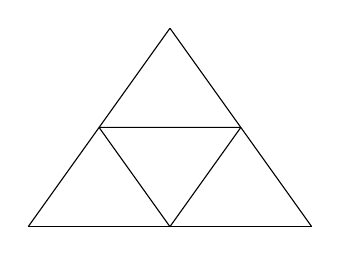
\begin{tikzpicture}[scale=0.9]
                    \coordinate (A) at (0,0);
                    \coordinate (B) at (2,0);
                    \coordinate (C) at (1,1.4);
                    \coordinate (D) at ($2*(B)$);
                    \coordinate (E) at ($(B)+(C)$);
                    \coordinate (F) at ($2*(C)$);

                    \draw[\colA, \width] (A) -- (B) -- (D);
                    \draw[\colA, \width] (C) -- (E);
                    \draw[\colB, \width] (B) -- (C);
                    \draw[\colB, \width] (D) -- (E) -- (F);
                    \draw[\colC, \width] (A) -- (C) -- (F);
                    \draw[\colC, \width] (B) -- (E);
                \end{tikzpicture}
            \end{center}
\end{frame}


\begin{frame}{Colouring as permutation}
    \onslide<2->{
        Consider tetrahedron \onslide<4->{with edge colouring}
    }
    \begin{center}
        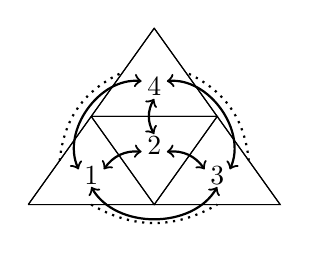
\begin{tikzpicture}[scale=0.8]
                \coordinate (A) at (0,0);
                \coordinate (B) at (2,0);
                \coordinate (C) at (1,1.4);
                \coordinate (D) at ($2*(B)$);
                \coordinate (E) at ($(B)+(C)$);
                \coordinate (F) at ($2*(C)$);
            \onslide<3->{
                \draw (A) -- (B) -- (D) -- (E) -- (F) -- (C) -- (E) -- (B) -- (C) -- (A);
                \node at (barycentric cs:A=1,B=1,C=1) {1};
                \node at (barycentric cs:B=1,C=1,E=1) {2};
                \node at (barycentric cs:B=1,D=1,E=1) {3};
                \node at (barycentric cs:C=1,E=1,F=1) {4};
                \draw[dotted,thick] ($(A)!0.5!(C)$) to[bend left] ($(C)!0.5!(F)$);
                \draw[dotted,thick] ($(A)!0.5!(B)$) to[bend right] ($(B)!0.5!(D)$);
                \draw[dotted,thick] ($(D)!0.5!(E)$) to[bend right] ($(E)!0.5!(F)$);
            }
            \onslide<5->{
                \draw[\colA, \width] (A) -- (B) -- (D);
                \draw[\colA, \width] (C) -- (E);
                \draw[\colB, \width] (B) -- (C);
                \draw[\colB, \width] (D) -- (E) -- (F);
                \draw[\colC, \width] (A) -- (C) -- (F);
                \draw[\colC, \width] (B) -- (E);
            }

            % Draw switching arrows
            \onslide<9-11>{
                \draw[<->,\colB, thick] (barycentric cs:A=1,B=2,C=2) to[bend left] (barycentric cs:B=2,C=2,E=1);
            }
            \onslide<10-11>{
                \draw[<->,\colB,thick] (barycentric cs:B=1,D=2,E=2) to[bend right=60] (barycentric cs:E=2,F=2,C=1);
            }
            \onslide<12>{
                \draw[<->,\colA,thick] (barycentric cs:A=2,B=2,C=1) to[bend right=60] (barycentric cs:B=2,D=2,E=1);
                \draw[<->,\colA,thick] (barycentric cs:C=2,E=2,B=1) to[bend left] (barycentric cs:C=2,E=2,F=1);
            }
            \onslide<13>{
                \draw[<->,\colC,thick] (barycentric cs:A=2,B=1,C=2) to[bend left=60] (barycentric cs:C=2,E=1,F=2);
                \draw[<->,\colC,thick] (barycentric cs:B=2,C=1,E=2) to[bend left] (barycentric cs:B=2,D=1,E=2);
            }
        \end{tikzpicture}
    \end{center}
    \onslide<6->{
        \textit{simplicial surface} $\Rightarrow$ \onslide<7->{at most two faces at each edge}
    
        \begin{itemize}
            \item<8->[$\leadsto$] every edge defines transposition of incident faces
            \item<11->[$\leadsto$] every colour class defines permutation of the faces
            \item<9-> \textcolor{\colB}{(1,2)}\onslide<10->{\textcolor{\colB}{(3,4)}}
                    \onslide<12->{, \textcolor{\colA}{(1,3)(2,4)}}
                    \onslide<13->{, \textcolor{\colC}{(1,4)(2,3)}}
            \item<14->[$\leadsto$] group theoretic considerations
                \begin{itemize}
                    \item<15-> The connected components of the surface correspond to 
                        \onslide<16->{the orbits of $\langle 
                            \textcolor{\colA}{\sigma_a}, 
                            \textcolor{\colB}{\sigma_b}, 
                            \textcolor{\colC}{\sigma_c}\rangle$ on
                        the faces}
                \end{itemize}
        \end{itemize}
    }
\end{frame}
         

\begin{frame}{How do faces fit together?}
    \onslide<2->{
        Consider a face of the surface \onslide<4->{and a neighbouring face}
    }

    \onslide<6->{
        The neighbour can be coloured in two ways:
    }
    \onslide<1->{
        \begin{center}
        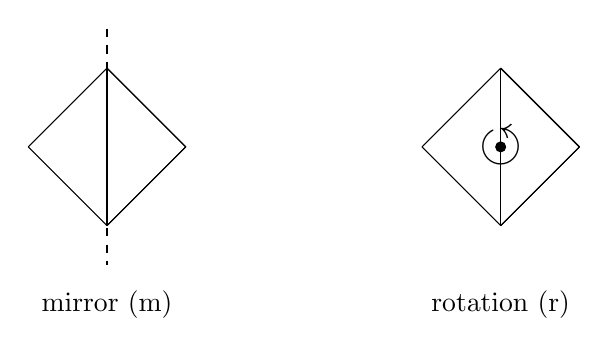
\begin{tikzpicture}
            % Numbers to determine drawing
            \def\x{1}
            \def\y{1}

            %      B
            %    / | \
            %   A  |  D
            %    \ | /
            %      C
            
            % First pair
            \begin{scope}
                \coordinate (A) at (0,0);
                \coordinate (B) at (\x,\y);
                \coordinate (C) at (\x,-\y);
                \coordinate (D) at (2*\x,0);

                \onslide<3->{
                    \draw[\colA,\width] (A) -- (B);
                    \draw[\colB,\width] (A) -- (C);
                    \draw[\colC,\width] (B) -- (C);
                }
                \onslide<5->{
                    \draw (B) -- (D) -- (C);
                }
                \onslide<7->{
                    \draw[\colA,\width] (B) -- (D);
                    \draw[\colB,\width] (C) -- (D);
                }
                \onslide<9->{
                    % Draw mirror line
                    \draw[dashed, thick] (\x,1.5*\y) -- (\x,-1.5*\y);
                    \node at (\x,-2*\y) {mirror (m)};
                }
            \end{scope}

            % Second pair
            \begin{scope}[xshift=5cm]
                \coordinate (A) at (0,0);
                \coordinate (B) at (\x,\y);
                \coordinate (C) at (\x,-\y);
                \coordinate (D) at (2*\x,0);

                \onslide<6->{
                    \draw[\colA,\width] (A) -- (B);
                    \draw[\colB,\width] (A) -- (C);
                    \draw[\colC,\width] (B) -- (C);
                    \draw (B) -- (D) -- (C);
                }
                \onslide<8->{
                    \draw[\colB,\width] (B) -- (D);
                    \draw[\colA,\width] (C) -- (D);
                }
                \onslide<10->{
                    % Draw rotation center and circle
                    \fill[black] (\x,0) circle (2pt);
                    \node[scale=2] at (\x,0) {$\circlearrowleft$};
                    \node at (\x,-2*\y) {rotation (r)};
                }
            \end{scope}
        \end{tikzpicture}
        \end{center}
    }
    \onslide<11->{
        This gives an \textbf{mr--assignment} for the edges.
    }

    \onslide<12->{
        Permutations and mr--assignment uniquely determine the surface.
    }
\end{frame}


\begin{frame}{Constructing surfaces from groups}
    \pause
    A general mr--assignment leads to complicated surfaces.
    
    \pause
    Simplification: edges of same colour have the same type

    \pause
    Example
        \begin{center}
            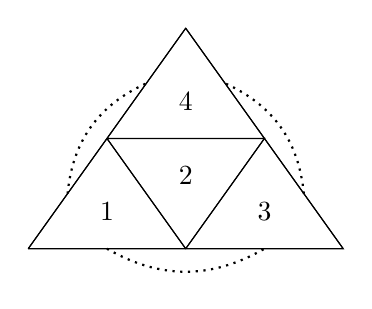
\begin{tikzpicture}
                \coordinate (A) at (0,0);
                \coordinate (B) at (2,0);
                \coordinate (C) at (1,1.4);
                \coordinate (D) at ($2*(B)$);
                \coordinate (E) at ($(B)+(C)$);
                \coordinate (F) at ($2*(C)$);

                \draw (A) -- (B) -- (D) -- (E) -- (F) -- (C) -- (E) -- (B) -- (C) -- (A);
                \node at (barycentric cs:A=1,B=1,C=1) {1};
                \node at (barycentric cs:B=1,C=1,E=1) {2};
                \node at (barycentric cs:B=1,D=1,E=1) {3};
                \node at (barycentric cs:C=1,E=1,F=1) {4};
                
                \draw[dotted,thick] ($(A)!0.5!(C)$) to[bend left] ($(C)!0.5!(F)$);
                \draw[dotted,thick] ($(A)!0.5!(B)$) to[bend right] ($(B)!0.5!(D)$);
                \draw[dotted,thick] ($(D)!0.5!(E)$) to[bend right] ($(E)!0.5!(F)$);

                \draw[\colA, \width] (A) -- (B) -- (D);
                \draw[\colA, \width] (C) -- (E);
                \draw[\colB, \width] (B) -- (C);
                \draw[\colB, \width] (D) -- (E) -- (F);
                \draw[\colC, \width] (A) -- (C) -- (F);
                \draw[\colC, \width] (B) -- (E);
            \end{tikzpicture}
        \end{center}
    \pause
    has an rrr--structure

    \pause
    The easiest structure is an mmm--structure.
\end{frame}


\begin{frame}{Covering}
    \pause
    We want to characterize surfaces where all edges are mirrors.
    \pause
    \begin{lem}
        A simplicial surface has an mmm--structure iff it covers a 
        single triangle\pause, i.\,e. there is an incidence--preserving
        map to the simplicial surface consisting of exactly one face.
    \end{lem}
    \pause
    Consider
        \begin{center}
            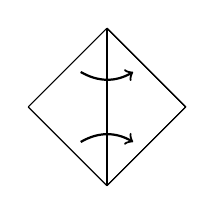
\begin{tikzpicture}
                \def\x{1}
                \def\y{1}

                \coordinate (A) at (0,0);
                \coordinate (B) at (\x,\y);
                \coordinate (C) at (\x,-\y);
                \coordinate (D) at (2*\x,0);

                    \draw[\colA,\width] (A) -- (B);
                    \draw[\colB,\width] (A) -- (C);
                    \draw[\colC,\width] (B) -- (C);
                    \draw (B) -- (D) -- (C);
                    \draw[\colA,\width] (B) -- (D);
                    \draw[\colB,\width] (C) -- (D);

                \def\mid{3}
                \def\near{5}
                \draw[->,thick] (barycentric cs:A=\mid,B=\near,C=1) to[bend right] (barycentric cs:B=\near,C=1,D=\mid);
                \draw[->,thick] (barycentric cs:A=\mid,B=1,C=\near) to[bend left] (barycentric cs:B=1,C=\near,D=\mid);
            \end{tikzpicture}
        \end{center}
    \begin{itemize}
        \pause
        \item[$\Rightarrow$] Unique map that preserves incidence
        \pause
        \item Covering pulls back a mirror--colouring of the triangle.
        \pause
        \item Mirror--colouring defines a map to the triangle.
    \end{itemize}
\end{frame}


\begin{frame}[fragile]{Construction from permutations}
    \onslide<2->{
    Start with three involutions \textcolor{\colA}{$\sigma_a$}, 
        \textcolor{\colB}{$\sigma_b$}, \textcolor{\colC}{$\sigma_c$}
        \onslide<3->{(like generators of a finite group)}
    }

    \onslide<4->{
    \begin{lem}
        There exists a coloured surface with the given involutions
        \onslide<5->{where all edges are mirror edges.}
    \end{lem}
    }

    \begin{itemize}
        \item<6-> The faces are the points moved by the involutions
        \item<7-> The edges are the cycles of the involutions
        \item<8-> The vertices are \onslide<11->{the orbits of 
            $\langle \textcolor{\colA}{\sigma_a}, 
            \textcolor{\colB}{\sigma_b} \rangle$
            on the faces} \onslide<12->{(for all pairs)}
    \end{itemize}

    \onslide<9->{
    \begin{center}
    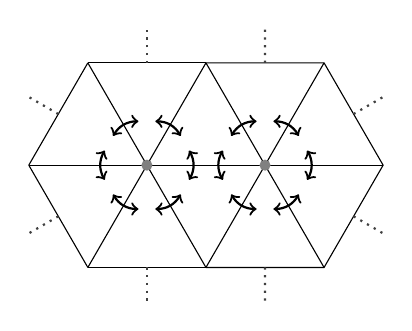
\begin{tikzpicture}
        %     P2 ---- P1 ---- Q3
        %    /  \    /  \   /  \
        %   /    \  /    \ /    \
        % P3 ---- Z ---- P0 ---- Q2
        %   \    /  \    /  \   /
        %    \  /    \  /    \ /
        %     P4 ---- P5 ---- Q1

        % Define the coordinates
        \def\rad{1.5}
        \coordinate (Z) at (0,0);
        \foreach \i in {0,1,2,3,4,5}
            \coordinate (P\i) at (60*\i:\rad);

        \foreach \i in {1,2,3}
            \coordinate (Q\i) at ($(P0) + (-120+60*\i:\rad)$);
        
        % Draw the circle around Z
        \foreach \i/\j in {0/1, 1/2, 2/3, 3/4, 4/5, 5/0}{
            \draw[\colC, \width] (P\i) -- (P\j);
        }

        % Draw the spokes of Z
        \foreach \i in {0,2,4}
            \draw[\colA,\width] (Z) -- (P\i);

        \foreach \i in {1,3,5}
            \draw[\colB,\width] (Z) -- (P\i);

        % Draw missing lines around P0
        \draw[\colB, \width] (P5) -- (Q1) -- (Q2) -- (Q3) -- (P1);
        \draw[\colA, \width] (Q1) -- (P0) -- (Q3);
        \draw[\colC, \width] (P0) -- (Q2);

        % Draw the continuations
        \foreach \p/\q/\z in {P1/P2/Z, P2/P3/Z, P3/P4/Z, P4/P5/Z, P5/Q1/P0, Q1/Q2/P0, Q2/Q3/P0, Q3/P1/P0}
            \draw[gray!50!black, dotted, thick] ($(\p)!0.5!(\q)$) -- (barycentric cs:\z=-0.5,\p=1,\q=1);

        % Draw the vertices
        \foreach \p in {Z,P0}
            \fill[gray] (\p) circle (2pt);

        % Draw the arc segments (center, outer, first, second, colour)
        \newcommand{\arcSeg}[5]{
            \draw[#5, thick, <->] (barycentric cs:#1=4,#2=2,#3=1) to[bend right] (barycentric cs:#1=4,#2=2,#4=1);
        }
        \onslide<10->{
        \arcSeg{Z}{P1}{P0}{P2}{\colB}
        \arcSeg{Z}{P2}{P1}{P3}{\colA}
        \arcSeg{Z}{P3}{P2}{P4}{\colB}
        \arcSeg{Z}{P4}{P3}{P5}{\colA}
        \arcSeg{Z}{P5}{P4}{P0}{\colB}
        \arcSeg{Z}{P0}{P5}{P1}{\colA}
        }

        \onslide<12->{
        \arcSeg{P0}{Q3}{Q2}{P1}{\colA}
        \arcSeg{P0}{P1}{Q3}{Z}{\colC}
        \arcSeg{P0}{Z}{P1}{P5}{\colA}
        \arcSeg{P0}{P5}{Z}{Q1}{\colC}
        \arcSeg{P0}{Q1}{P5}{Q2}{\colA}
        \arcSeg{P0}{Q2}{Q1}{Q3}{\colC}
        }
    \end{tikzpicture}
    \end{center}
    }
\end{frame}


\begin{frame}{Construction example}
    \onslide<2->{ $\textcolor{\colA}{\sigma_a} = \textcolor{\colA}{(1,2)(3,4)(5,6)(7,8)}$\\ }
    \onslide<3->{ $\textcolor{\colB}{\sigma_b} = \textcolor{\colB}{(1,4)(2,3)(5,8)(6,7)}$\\ }
    \onslide<4->{ $\textcolor{\colC}{\sigma_c} = \textcolor{\colC}{(1,5)(2,6)(3,7)(4,8)}$\\ }

    \begin{center}
    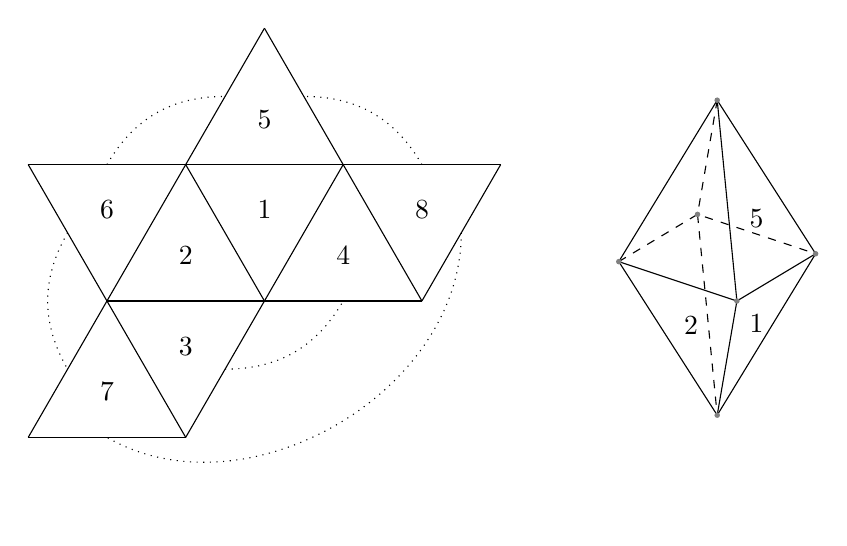
\begin{tikzpicture}
        % Coordinates
        \coordinate (Z) at (0,0);
        \foreach \i in {0,1,2,3,4}
            \coordinate (P\i) at (60*\i:2);
        \foreach \i/\j in {0/1, 1/2, 2/3, 3/4}
            \coordinate (Q\i\j) at ($(P\i)+(P\j)$);

        % 1
        \onslide<5->{
            \node at (barycentric cs:Z=1,P1=1,P2=1) {1};
            \draw[\colA,\width] (Z) -- (P2);
            \draw[\colB,\width] (Z) -- (P1);
            \draw[\colC,\width] (P1) -- (P2);
        }

        % 2
        \onslide<6->{
            \node at (barycentric cs:Z=1,P2=1,P3=1) {2};
            \draw[\colB,\width] (Z) -- (P3);
            \draw[\colC,\width] (P2) -- (P3);
        }

        % 4
        \onslide<7->{
            \node at (barycentric cs:Z=1,P0=1,P1=1) {4};
            \draw[\colA,\width] (Z) -- (P0);
            \draw[\colC,\width] (P0) -- (P1);
        }

        % 5
        \onslide<8->{
            \node at (barycentric cs:P1=1,P2=1,Q12=1) {5};
            \draw[\colB,\width] (P1) -- (Q12);
            \draw[\colA,\width] (P2) -- (Q12);
        }

        % 3
        \onslide<9->{
            \node at (barycentric cs:Z=1,P3=1,P4=1) {3};
            \draw[\colC,\width] (P3) -- (P4);
            \draw[\colA,\width] (Z) -- (P4);
        }
        \onslide<10->{
            \draw[\colA,\width,dotted] ($(Z)!0.5!(P4)$) to[bend right] ($(Z)!0.5!(P0)$);
        }

        % 6
        \onslide<11->{
            \node at (barycentric cs:P2=1,P3=1,Q23=1) {6};
            \draw[\colA,\width] (P2) -- (Q23);
            \draw[\colA,\width,dotted] ($(P2)!0.5!(Q23)$) to[bend left] ($(P2)!0.5!(Q12)$);
            \draw[\colB,\width] (P3) -- (Q23);
        }

        % 7
        \onslide<12->{
            \node at (barycentric cs:P3=1,P4=1,Q34=1) {7};
            \draw[\colB,\width] (P3) -- (Q34);
            \draw[\colB,\width,dotted] ($(P3)!0.5!(Q23)$) to[bend right] ($(P3)!0.5!(Q34)$);
            \draw[\colA,\width] (P4) -- (Q34);
        }

        % 8
        \onslide<13->{
            \node at (barycentric cs:P0=1,P1=1,Q01=1) {8};
            \draw[\colB,\width] (P1) -- (Q01);
            \draw[\colB,\width,dotted] ($(P1)!0.5!(Q01)$) to[bend right] ($(P1)!0.5!(Q12)$);
            \draw[\colA,\width] (P0) -- (Q01);
        }
        \onslide<14->{
            \draw[\colA,\width,dotted] ($(P0)!0.5!(Q01)$) to[bend left=60] ($(P4)!0.5!(Q34)$);
        }

        \begin{scope}[xshift=6cm]
            % Coordinates of octahedron
                \def\len{2} % The length of the base
                \def\h{1}   % \h*\len is the hight of the apex above the 
                            % center of the square
                \coordinate (Mid) at (0,0);
                \coordinate (Right) at (0.5*\len,0.3*\len);
                \coordinate (Left) at (-0.75*\len,0.25*\len);
                \coordinate (Back) at ($(Right)+(Left)$);
                \coordinate (Center) at ($(Left)!0.5!(Right)$);
                \coordinate (Up) at ($(Center)+(0,\h*\len)$);
                \coordinate (Down) at ($(Center)+(0,-\h*\len)$);

                \onslide<15->{
                    \draw[\colA,\width] (Up) -- (Mid) -- (Down);
                    \draw[\colA,\width,dashed] (Up) -- (Back) -- (Down);
                    \draw[\colB,\width] (Up) -- (Right) -- (Down) -- (Left) -- cycle;
                    \draw[\colC,\width] (Left) -- (Mid) -- (Right);
                    \draw[\colC,\width,dashed] (Left) -- (Back) -- (Right);

                    \node at (barycentric cs:Mid=1,Down=1,Right=1) {1};
                    \node at (barycentric cs:Mid=1,Down=1,Left=1) {2};
                    \node at (barycentric cs:Mid=1,Up=1,Right=1) {5};
                    %\node at (barycentric cs:Mid=1,Up=1,Left=1) {6};
                    
                    % Vertices to hide drawing problems in edge meetings
                    \foreach \p in {Mid,Right,Left,Back,Up,Down}
                        \fill[gray] (\p) circle (1pt);
                }
        \end{scope}
    \end{tikzpicture}
    \end{center}
\end{frame}



%%%%%%%%%%%%%%%%%%%%%%%%%%%%%%%%%%%%%%%%%%%%%%%%%%%%%%%%%%%%%%
%%
%%    Third section
%%
\section{Abstract folding}
\frame{\tableofcontents[currentsection]}

\begin{frame}{What kind of folding?}
    \pause
    There are many different kinds of folding (e.\,g. Origami)

    \pause
    Here:
    \begin{itemize}
        \pause
        \item Folding of surface in $\R^3$
        \pause
        \item Fold only at given edges (no introduction of new folding edges)
        \pause
        \item Folding should be rigid (no curvature)
    \end{itemize}

    \pause
    Goal: Classify possible folding patterns (given a net)

    \pause
    \begin{center}
        \only<1-7>{
            \phantom{ 
                \movie[ height = 0.4\textwidth, width = 0.4\textwidth, autostart, loop ]{}{TorusNetz.mp4}
            }
        }
        \only<8>{
            \movie[ height = 0.4\textwidth, width = 0.4\textwidth, autostart, loop ]{}{TorusNetz.mp4}
        }
    \end{center}

\end{frame}


\begin{frame}{Why are embeddings hard?}
    \pause
    Ideally, we would like to have embeddings.
    
    \pause
    But we want to define folding independently from an embedding, since:

    \begin{itemize}
        \pause
        \item They are very hard to compute (even for small examples)
        \pause
        \item We can only show foldability for specific small examples
            \begin{itemize}
                \pause
                \item Usually using regularity (like crystallographic symmetry)
                \pause
                \item No general method
            \end{itemize}
        \pause
        \item It is very hard to define iterated folding in an embedding
    \end{itemize}

    \pause
    \begin{center}
        \only<1-8>{
            \phantom{
                \movie[ height = 0.4\textwidth, width = 0.4\textwidth, autostart, loop ]{}{TorusNetz.mp4}
            }
        }
        \only<9>{
            \movie[ height = 0.4\textwidth, width = 0.4\textwidth, autostart, loop ]{}{TorusNetz.mp4}
        }
    \end{center}

\end{frame}


\begin{frame}{Folding without embedding}
    \pause
    Central idea:
    \begin{itemize}
        \pause
        \item Don't model folding process (needs embedding)
        \pause
        \item Describe starting and final folding state
            \begin{itemize}
                \pause
                \item Only consider changes in the topology
                    \pause (like identification of faces)
                \pause
                \item allows abstraction from embedding
            \end{itemize}
    \end{itemize}

    % Use pentagon-flippy to illustrate incidence rigidity

    \pause
    $\leadsto$ Incidence geometry (polygonal complex/surface)

    \begin{itemize}
        \pause
        \item Captures some folding restrictions \pause (rigidity of tetrahedron)
        \pause
        \item Still needs a lot of refinement
    \end{itemize}
\end{frame}

\newcommand{\colFaceA}{\colorFaceA}
\newcommand{\colFaceB}{\colorFaceB}
\newcommand{\colFaceC}{\colorFaceC}

\begin{frame}{Important properties of folding}
    \begin{itemize}
        \item<2-> The class of surfaces is not closed under folding
        \item<3-> Folding can be undone by \textit{unfolding}
        \item<4-> Identification of two faces might force identification of two other faces
            \begin{itemize}
                \item<7-> Can apply to arbitrary many faces 
                \item<10-> The forced identification is not unique
                \item<14->[$\Rightarrow$] Identify only two faces at a time
            \end{itemize}
    \end{itemize}

    \begin{overlayarea}{\textwidth}{0.3\textwidth}
        \begin{center}
            \only<5-7,14|handout:0>{
                % First identification
                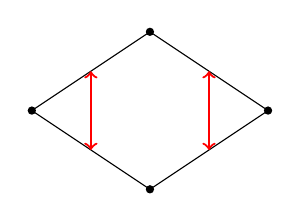
\begin{tikzpicture}
                    \def\Hdist{1.5}
	    	    \def\Vdist{1}
			
		    \coordinate (A) at (-\Hdist,0);
		    \coordinate (B) at (0,\Vdist);
		    \coordinate (C) at (\Hdist,0);
		    \coordinate (D) at (0,-\Vdist);
                    \draw (A) -- (B) -- (C) -- (D) -- cycle;

		    \foreach \p in {A,B,C,D}
		        \fill [\vertexColor] (\p) circle (1.5pt);
		    \draw [<->,\colorRed,thick] ($(B)!0.5!(A)$) -- ($(D)!0.5!(A)$);
                    \uncover<6-7>{
                        \draw[<->,\colorRed,thick] ($(B)!0.5!(C)$) -- ($(D)!0.5!(C)$);
                    }
                \end{tikzpicture}
            }

            % Arbitrary many faces
            \only<8-10|handout:0>{
                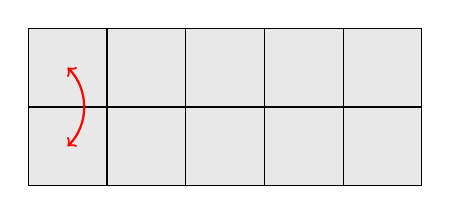
\begin{tikzpicture}
		    \foreach \i/\j in {1/0, 2/1, 3/2, 4/3, 5/4}
		    {
		        \filldraw [fill=black!9!white] (\j,0) -- (\i,0) -- (\i,1) -- (\j,1) -- cycle;
		        \filldraw [fill=black!9!white] (\j,0) -- (\i,0) -- (\i,-1) -- (\j,-1) -- cycle;
		    }
                    \uncover<9-10>{
                        \draw [\colorRed,<->,thick] (0.5,0.5) to [out=-45,in=45] (0.5,-0.5);
	            }
                \end{tikzpicture}
            }

            % Picture of non-uniqueness:
            \only<11-13|handout:1>{
                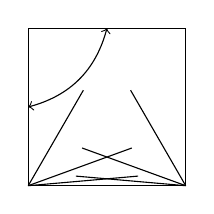
\begin{tikzpicture}
                    \def\len{2}
                    \def\fak{0.7}
                    \coordinate (A) at (0,0);
                    \coordinate (B) at (\len,0);
                    \coordinate (C) at (\len,\len);
                    \coordinate (D) at (0,\len);

                    \draw (A) -- (B) -- (C) -- (D) -- cycle;
                    \uncover<11>{
                        \draw[\colFaceB] (A) -- (60:\fak*\len);
                        \draw[\colFaceA] (B) -- ($(B)+(120:\fak*\len)$);
                    }

                    \draw[<->] ($(A)!0.5!(D)$) to[bend right] ($(D)!0.5!(C)$);

                    \uncover<12|handout:0>{
                        \draw[\colFaceB] (A) -- (5:\fak*\len);
                        \draw[\colFaceA] (B) -- ($(B)+(160:\fak*\len)$);
                    }

                    \uncover<13|handout:0>{
                        \draw[\colFaceB] (A) -- (20:\fak*\len);
                        \draw[\colFaceA] (B) -- ($(B)+(175:\fak*\len)$);
                    }
                \end{tikzpicture}
            }
            % 11: general picture
            % 12: First possible fold
            % 13: Second possible fold

            % Anomaly-picture
            \only<15-|handout:2>{
                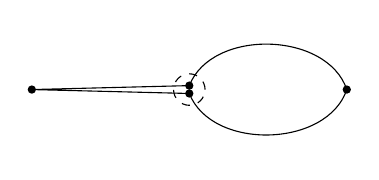
\begin{tikzpicture}
		    \def\r{2}	
		    \def\eps{0.05}
				
		    \coordinate (A) at (-\r,0);
		    \coordinate (B) at (0,\eps);
		    \coordinate (C) at (\r,0);
		    \coordinate (D) at (0,-\eps);
			
		    \draw (D) -- (A) -- (B);
		    \draw (B) to [bend left=70] (C);
		    \draw (D) to [bend right=70] (C);
			
		    \foreach \point in {A,B,C,D}
		        \fill [\vertexColor] (\point) circle (1.5pt);
				
		    \draw [dashed] (0,0) circle (0.2);
                \end{tikzpicture}
            }
        \end{center}
    \end{overlayarea}
\end{frame}


\begin{frame}{How to define abstract folding?}
    \uncover<2->{We need to define two structures:}
    \begin{enumerate}
        \item<3-> A folding state
            \begin{itemize}
                \item<5-> Based on polygonal complexes
                \item<6-> Describe ``is folded together" by an equivalence relation
                \item<7-> Describe order of faces in folding state
            \end{itemize}
        \item<4-> The folding steps
            \begin{itemize}
                \item<8-> Only two faces at a time
                \item<9-> Explain ``unordered folding" (e.\,g. covering)
                \item<10-> Modify to include face order relations
            \end{itemize}
    \end{enumerate}
\end{frame}


\begin{frame}{Unordered Folding (Covering)}
    \begin{center}
        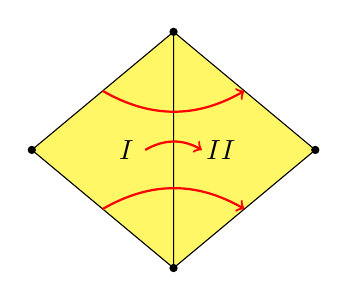
\begin{tikzpicture}
            \def\xOff{1.8}
            \def\yOff{1.5}

            %     B
            %   / | \
            % A   |   C
            %   \ | /
            %     D
            \coordinate (A) at (-\xOff,0);
            \coordinate (B) at (0,\yOff);
            \coordinate (C) at (\xOff,0);
            \coordinate (D) at (0,-\yOff);

            \uncover<3->{
                \filldraw[face] (A) -- (B) -- (D) -- cycle;
                \node at (barycentric cs:A=1,B=1,D=1) {$I$};
                \filldraw[face] (B) -- (C) -- (D) -- cycle;
                \node at (barycentric cs:B=1,C=1,D=1) {$II$};

                \foreach \p in {A,B,C,D}
                    \fill[\vertexColor] (\p) circle (1.5pt);
            }

            \uncover<5-7|handout:1>{
                \draw[\colorRed,thick,->] (barycentric cs:A=1,B=2,D=2) to[bend left] (barycentric cs:B=2,C=1,D=2);
                \draw[\colorRed,thick,->] ($(A)!0.5!(B)$) to[bend right] ($(B)!0.5!(C)$);
                \draw[\colorRed,thick,->] ($(A)!0.5!(D)$) to[bend left] ($(D)!0.5!(C)$);
            }
        \end{tikzpicture}
    \end{center}

    \begin{overprint}
        \onslide<1-7|handout:1>
        
        \uncover<2-7>{
            Why do we need more than a polygonal complex?
        }

        \uncover<4-7>{
            Naive folding definition: surjective map that respects incidence
        }

        \uncover<6-7>{
            Problem: Can't be unfolded
        }

        \uncover<7>{
            $\Rightarrow$ Folding state should not forget original structure
        }


        \onslide<8-16|handout:2>

        \uncover<8-16>{
            Represent folding by equivalence relation
            \begin{itemize}
                \item<9-> Separate relation on vertices, edges and faces
                \item<10-> Two elements are equivalent if they are folded together
                \item<11-> If two edges are equivalent, 
                    \uncover<12->{then their vertices have to be as well}
                    \uncover<13->{(likewise for faces)}
                \item<14-> The vertices of an edge are not equivalent
                    \uncover<15->{(likewise for faces)}
                \item<16->[$\Rightarrow$] Unordered folding is coarsening of equivalence relation
            \end{itemize}
        }
    \end{overprint}
\end{frame}


\begin{frame}{How does folding work?}
    \begin{enumerate}
        \item<2-> Choose two faces that are not folded together
        \item<4-> Choose how to identify them \uncover<6->{(like $I \sim II$ and $1 \sim 4$)}
        \item<7-> Add those pairs to the equivalence relation
    \end{enumerate}

    \begin{center}
        \begin{tikzpicture}
            \def\xOff{1.8}
            \def\yOff{1.5}

            %     B
            %   / | \
            % A   |   C
            %   \ | /
            %     D
            \uncover<3->{
                \coordinate[label={[vertex]left:1}] (A) at (-\xOff,0);
                \coordinate[label={[vertex]above:2}] (B) at (0,\yOff);
                \coordinate[label={[vertex]right:4}] (C) at (\xOff,0);
                \coordinate[label={[vertex]below:3}] (D) at (0,-\yOff);

                \filldraw[face] (A) -- (B) -- (D) -- cycle;
                \node at (barycentric cs:A=1,B=1,D=1) {$I$};
                \filldraw[face] (B) -- (C) -- (D) -- cycle;
                \node at (barycentric cs:B=1,C=1,D=1) {$II$};

                \foreach \p in {A,B,C,D}
                    \fill[\vertexColor] (\p) circle (1.5pt);
            }

            \uncover<5->{
                \draw[\colorRed,thick,->] (barycentric cs:A=1,B=2,D=2) to[bend left] (barycentric cs:B=2,C=1,D=2);
                \draw[\colorRed,thick,->] ($(A)!0.5!(B)$) to[bend right] ($(B)!0.5!(C)$);
                \draw[\colorRed,thick,->] ($(A)!0.5!(D)$) to[bend left] ($(D)!0.5!(C)$);
            }
        \end{tikzpicture}
    \end{center}

    \uncover<8->{Only restriction:}

    \uncover<9->{Two vertices in an edge can't be identified}
    \uncover<10->{(slightly generalized)}
\end{frame}


\begin{frame}[fragile]{Limitation of unordered folding}
    \pause
    We can't work with ordering of faces:
    \pause
    \begin{center}
        
\begin{tikzpicture}

            \newcommand{\plane}[3]{
                \def\len{1.5}
                \def\back{0.75}
                \def\xOff{0.5}
                \def\nOff{-0.3}
                
                \coordinate (Down) at (#1*\xOff,0);
                \coordinate (Up) at (#1*\xOff,\len);
                \coordinate (Back) at (\back*\xOff,\back*\xOff);

                \fill[#2] (Down) -- ($(Down)+(Back)$) -- ($(Up)+(Back)$) -- (Up) -- cycle;
                \node[#2] at (#1*\xOff,\nOff) {#3};
            }

            \plane{0}{\colFaceB}{1}
            \plane{1}{\colFaceA}{2}
            \plane{2}{\colFaceC}{3}

            % Second lines
            \begin{scope}[xshift=4cm]
                \plane{0}{\colFaceB}{1}
                \plane{1}{\colFaceC}{3}
                \plane{2}{\colFaceA}{2}
            \end{scope}
        \end{tikzpicture}
    \end{center}

    \pause
    Adding a linear order on each face equivalence class
    \pause is not enough:
    \pause
    \begin{center}
        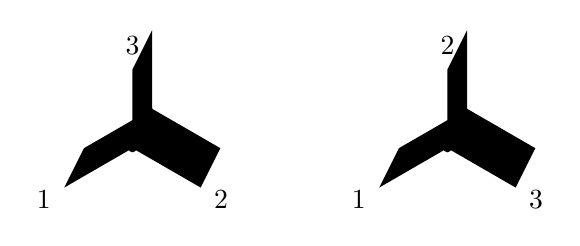
\begin{tikzpicture}

            \newcommand{\plane}[3]{
                \def\len{1}
                \def\nScale{1.3}

                \coordinate (Back) at (0.25*\len,0.5*\len);
                \fill[#2] (0,0) -- (#1:\len) -- +(Back) -- (Back) -- cycle; 
                \node[#2] at (#1:\nScale*\len) {#3};
                \draw (0,0) -- (Back);
            }

            \plane{210}{\colFaceA}{1}
            \plane{-30}{\colFaceB}{2}
            \plane{90}{\colFaceC}{3}

            \fill (0,0) circle (1.5pt);

            \begin{scope}[xshift=4cm]
                \plane{210}{\colFaceA}{1}
                \plane{-30}{\colFaceC}{3}
                \plane{90}{\colFaceB}{2}

                \fill (0,0) circle (1.5pt);
            \end{scope}
        \end{tikzpicture}
    \end{center}

    \pause
    $\leadsto$ define order of faces around edges
    \pause
    (we will skip the details)
\end{frame}


\begin{frame}{Folding complex}
    \pause
    \begin{defi}
        A \textbf{folding complex}
        \pause
        is a polygonal complex together with
        \begin{enumerate}
            \pause
            \item An equivalence relation on vertices, edges and faces
                \pause (``is folded together")
            \pause
            \item A linear ordering on each face equivalence class
            \pause
            \item A cyclical ordering of the faces around each edge equivalence class
        \end{enumerate}
        \pause
        such that the orderings are compatible
        \pause
        (in an appropriate sense).
    \end{defi}

    \pause
    To identify faces with each other, we have to combine those orderings.
    \begin{itemize}
        \pause
        \item linear orderings get concatenated
        \pause
        \item cyclical orderings are opened at one point
            \pause
            and combined
        \pause
        \item[!!] compatibility is not easily transfered,
            \pause
            but can be calculated
    \end{itemize}

\end{frame}


\begin{frame}[fragile]{Changed definition of folding}
    \begin{overprint}
        \only<2-4|handout:0>{Before (no ordering):}
        \only<5->{Folding with ordering:}
    \end{overprint}

    \begin{enumerate}
        \item<3-> Choose two faces that are not folded together
        \item<4-> Choose how to identify them and extend the equivalence relation
        \item<9-> Choose the sides of the faces that will meet
            \uncover<10->{and modify the orderings}
    \end{enumerate}

    \uncover<6->{
        $\leadsto$ Each face has two sides
    }

    \begin{center}
        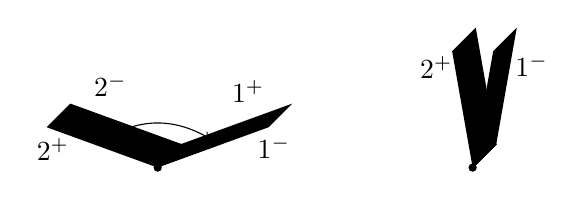
\begin{tikzpicture}
            \def\len{1.5}
            \def\wA{20}
            \def\wB{160}
            \def\nOff{10}

            % angle, colour
            \newcommand{\plane}[2]{
                \coordinate (Out) at (#1:\len);
                \coordinate (Back) at (0.2*\len,0.2*\len);

                \fill[#2] (0,0) -- (Out) -- +(Back) -- (Back) -- cycle;
                \draw (0,0) -- (Back);
            }

            \uncover<7->{
                \plane{\wA}{\colFaceA}
                \node[\colFaceA] at (\wA+2*\nOff:\len) {$1^+$};
                \node[\colFaceA] at (\wA-\nOff:\len) {$1^-$};

                \plane{\wB}{\colFaceB}
                \node[\colFaceB] at (\wB+\nOff:0.9*\len) {$2^+$};
                \node[\colFaceB] at (\wB-4*\nOff:0.8*\len) {$2^-$};

                \fill (0,0) circle (1.5pt);
            }

            \uncover<8->{
                \draw[<->] (\wB-\nOff: 0.5*\len) to[bend left] (\wA+\nOff:0.5*\len);
            }

            \begin{scope}[xshift=4cm]
                \uncover<8->{
                    \def\wA{80}
                    \def\wB{100}

                    \plane{\wB}{\colFaceB}
                    \node[\colFaceB] at (\wB+\nOff:0.9*\len) {$2^+$};
                    
                    \plane{\wA}{\colFaceA}
                    \node[\colFaceA] at (\wA-2*\nOff:\len) {$1^-$};

                    \fill (0,0) circle (1.5pt);
                }
            \end{scope}

        \end{tikzpicture}
    \end{center}

    \uncover<11->{
        $\Rightarrow$ Define folding by two face sides (\textbf{folding plan})
    }

    \uncover<12->{
        $\leadsto$ Allows reversible (un)folding
    }
\end{frame}


\begin{frame}{Structure of multiple foldings}
    \uncover<2->{
        With folding plans we can perform the same folding in different folding complexes
    }
    \begin{center}
        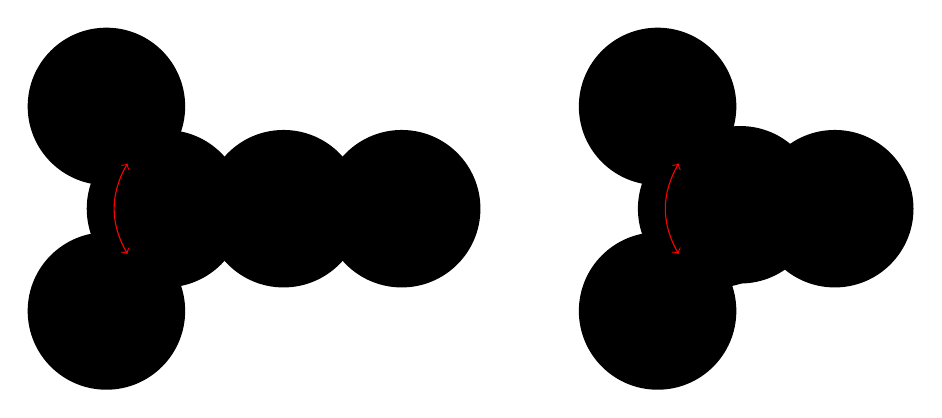
\begin{tikzpicture}
            \def\len{1.5}
            \def\off{10}

            %  B
            %   \
            %    Z -- C -- D
            %   /
            %  A
            \begin{scope}
                \coordinate (Z) at (0,0);
                \coordinate (A) at (-120:\len);
                \coordinate (B) at (120:\len);
                \coordinate (C) at (\len,0);
                \coordinate (D) at (2*\len,0);

                \uncover<3->{
                    \foreach \p/\q in {Z/A,Z/B,Z/C,C/D}
                        \draw (\p) -- (\q);
                    \foreach \p in {Z,A,B,C,D}
                        \fill[\vertexColor] (\p) circle (\vSize);
                }
                \uncover<5->{
                    \draw[\colorRed,<->] (120+\off:0.5*\len) to[bend right] (-120-\off:0.5*\len);
                }
            \end{scope}

            \begin{scope}[xshift=7cm]
                \def\pOff{0.05}

                \coordinate (Z) at (0,0);
                \coordinate (A) at (-120:\len);
                \coordinate (B) at (120:\len);
                \coordinate (C) at (\len,0);
                \coordinate (D) at (0.2*\len,\pOff);

                \uncover<4->{
                    \draw (A) -- (Z) -- (B);
                    \draw ($(Z)+(0,-\pOff)$) -- ($(C)+(0,-\pOff)$);
                    \draw ($(C)+(0,\pOff)$) -- (D);
                    \foreach \p in {A,B,Z,C,D}
                        \fill[\vertexColor] (\p) circle (\vSize);
                }
                \uncover<6->{
                    \draw[\colorRed,<->] (120+\off:0.5*\len) to[bend right] (-120-\off:0.5*\len);
                }
            \end{scope}
        \end{tikzpicture}
    \end{center}

    \uncover<7->{
        $\leadsto$ more structure on the set of possible foldings
    }
\end{frame}


\begin{frame}{Folding graph}
    \begin{itemize}
        \item<2->Vertices are folding complexes (modelling folding states)
        \item<3->Edges are folding plans connecting two folding complexes
    \end{itemize}

    \begin{center}
        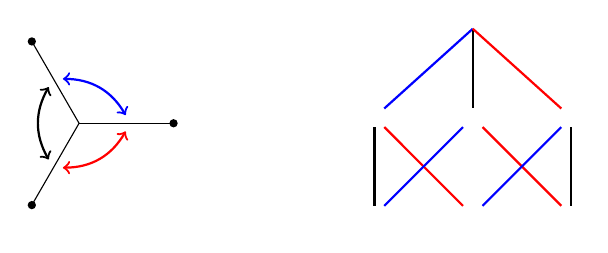
\begin{tikzpicture}[graphEdge/.style={thick}]
            \def\len{1.2}
            \def\off{10}

            \coordinate (Z) at (0,0);
            \foreach \i in {0,1,2}
                \coordinate (P\i) at (120*\i:\len);

            \uncover<4->{
                \foreach \i in {0,1,2}{
                    \draw (Z) -- (P\i);
                    \fill[\vertexColor] (P\i) circle (1.5pt);
                }
            }

            \def\fgA{\colorGraphB}
            \def\fgB{\colorGraphA}
            \def\fgC{\colorGraphC}
            \uncover<5->{
                \draw[graphEdge, \fgA,<->] (\off:0.5*\len) to[bend right] (120-\off:0.5*\len); 
                \draw[graphEdge, \fgB,<->] (120+\off:0.5*\len) to[bend right] (240-\off:0.5*\len);
                \draw[graphEdge, \fgC,<->] (-120+\off:0.5*\len) to[bend right] (-\off:0.5*\len);
            }

            % Second part
            \begin{scope}[xshift=5cm]
                \coordinate (Top) at (0,\len);
                \node (Mid) [below=of Top] {};
                \node (MidLeft) [left=of Mid] {};
                \node (MidRight) [right=of Mid] {};
                \node (DownLeft) [below=of MidLeft] {};
                \node (Down) [below=of Mid] {};
                \node (DownRight) [below=of MidRight] {};

                \uncover<6->{
                    \draw[graphEdge, \fgA] (Top) -- (MidLeft);
                    \draw[graphEdge, \fgB] (Top) -- (Mid);
                    \draw[graphEdge, \fgC] (Top) -- (MidRight);
                }
                \uncover<7->{
                    \draw[graphEdge, \fgB] (MidLeft) -- (DownLeft);
                    \draw[graphEdge, \fgC] (MidLeft) -- (Down);
                }
                \uncover<8->{
                    \draw[graphEdge, \fgA] (Mid) -- (DownLeft);
                    \draw[graphEdge, \fgC] (Mid) -- (DownRight);
                    \draw[graphEdge, \fgA] (MidRight) -- (Down);
                    \draw[graphEdge, \fgB] (MidRight) -- (DownRight);
                }
            \end{scope}
        \end{tikzpicture}
    \end{center}

    % Second diagram
    \begin{center}
        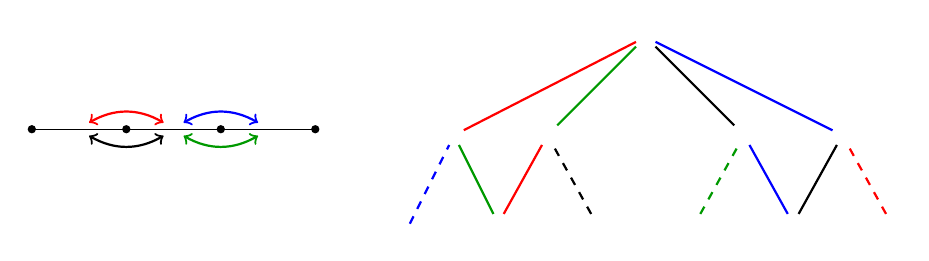
\begin{tikzpicture}[graphEdge/.style={thick}]
            \def\fgA{\colorGraphAlpha}
            \def\fgB{\colorGraphBeta}
            \def\fgC{\colorGraphGamma}
            \def\fgD{\colorGraphDelta}

            % First picture
            \def\len{1.2}
            \def\off{10}
            \def\scal{0.4}

            \foreach \i in {0,1,2,3}
                \coordinate (P\i) at (\i*\len,0);

            \uncover<9->{
                \draw (P0) -- (P1) -- (P2) -- (P3);
                \foreach \i in {0,1,2,3}
                    \fill[\vertexColor] (P\i) circle (1.5pt);
            }

            \uncover<10->{
                \draw[graphEdge, \fgA,<->] ($(P1)+(180-\off:\scal*\len)$) to[bend left] ($(P1)+(\off:\scal*\len)$);
                \draw[graphEdge, \fgB,<->] ($(P1)+(180+\off:\scal*\len)$) to[bend right] ($(P1)+(-\off:\scal*\len)$);
                \draw[graphEdge, \fgC,<->] ($(P2)+(180-\off:\scal*\len)$) to[bend left] ($(P2)+(\off:\scal*\len)$);
                \draw[graphEdge, \fgD,<->] ($(P2)+(180+\off:\scal*\len)$) to[bend right] ($(P2)+(-\off:\scal*\len)$);
            }

            \begin{scope}[xshift=6cm]
                \coordinate (B1) at (-\len,-\len);
                \foreach \i/\j in {1/2,2/3,3/4,4/5,5/6}{
                    \node (B\j) [right=of B\i] {};
                    \coordinate (H\i\j) at ($(B\i)!0.5!(B\j)$);
                    \node (M\i\j) [above=of H\i\j] {};
                }

                \node (Top) [above=of M34] {};

                \uncover<11->{
                    \draw[graphEdge, \fgA] (Top) -- (M12);
                    \draw[graphEdge, \fgB] (Top) -- (M45);
                    \draw[graphEdge, \fgC] (Top) -- (M56);
                    \draw[graphEdge, \fgD] (Top) -- (M23);
                }

                \uncover<12->{
                    \draw[graphEdge, \fgD] (B2) -- (M12);
                    \draw[graphEdge, \fgA] (B2) -- (M23);
                    \draw[graphEdge, \fgB] (B5) -- (M56);
                    \draw[graphEdge, \fgC] (B5) -- (M45);
                }

                \uncover<13->{
                    \draw[graphEdge, \fgC,dashed] (B1) -- (M12);
                }

                \uncover<14->{
                    \draw[graphEdge, \fgB,dashed] (B3) -- (M23);
                    \draw[graphEdge, \fgD,dashed] (B4) -- (M45);
                    \draw[graphEdge, \fgA,dashed] (B6) -- (M56);
                }
            \end{scope}
        \end{tikzpicture}
    \end{center}
\end{frame}


\begin{frame}{Drawback of folding plans}
    \uncover<2->{
        Some foldings that ``should" be the same, aren't:
    }
    \begin{center}
        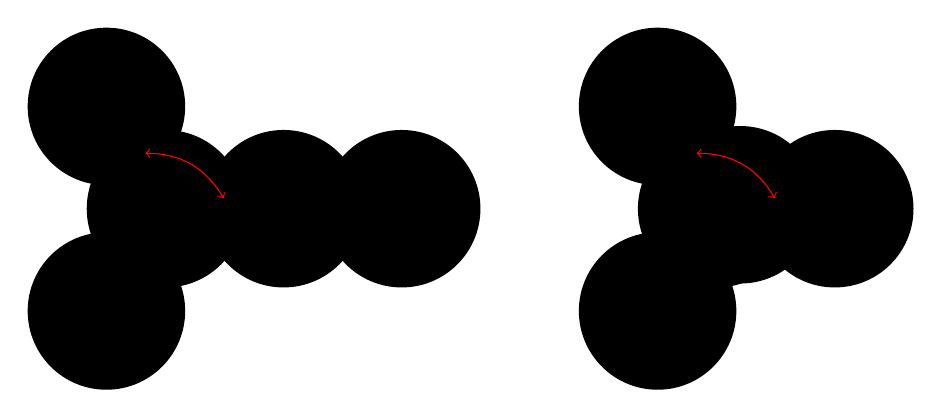
\begin{tikzpicture}
            \def\len{1.5}
            \def\off{10}

            %  B
            %   \
            %    Z -- C -- D
            %   /
            %  A
            \begin{scope}
                \coordinate (Z) at (0,0);
                \coordinate (A) at (-120:\len);
                \coordinate (B) at (120:\len);
                \coordinate (C) at (\len,0);
                \coordinate (D) at (2*\len,0);

                \uncover<3->{
                    \foreach \p/\q in {Z/A,Z/B,Z/C,C/D}
                        \draw (\p) -- (\q);
                    \foreach \p in {Z,A,B,C,D}
                        \fill[\vertexColor] (\p) circle (\vSize);
                }
                \uncover<5->{
                    \draw[\colorRed,<->] (120-\off:0.5*\len) to[bend left] (\off:0.5*\len);
                }
            \end{scope}

            \begin{scope}[xshift=7cm]
                \def\pOff{0.05}

                \coordinate (Z) at (0,0);
                \coordinate (A) at (-120:\len);
                \coordinate (B) at (120:\len);
                \coordinate (C) at (\len,0);
                \coordinate (D) at (0.2*\len,\pOff);

                \uncover<4->{
                    \draw (A) -- (Z) -- (B);
                    \draw ($(Z)+(0,-\pOff)$) -- ($(C)+(0,-\pOff)$);
                    \draw ($(C)+(0,\pOff)$) -- (D);
                    \foreach \p in {A,B,Z,C,D}
                        \fill[\vertexColor] (\p) circle (\vSize);
                }
                \uncover<6->{
                    \draw[\colorRed,<->] (120-\off:0.5*\len) to[bend left] (\off:0.5*\len);
                }
            \end{scope}
        \end{tikzpicture}
    \end{center}


    \begin{itemize}
        \item<7->[$\Rightarrow$]If you know the folding structure of a small complex,
            \uncover<8->{you can't easily find the folding structure of an extended complex}
        \item<9->[$\leadsto$]Folding plans are not optimal to model folding.
    \end{itemize}
\end{frame}





\begin{frame}{Questions?}
    
\end{frame}

\end{document}
